\graphicspath{{./figures/}}
\title{sandboxing}
\date{}
\begin{document}
\begin{frame}
    \titlepage
\end{frame}

\newcommand{\amp}{\textampersand}

\begin{frame}{last time (1)}
    \begin{itemize}
    \item Rust general syntax:
        \begin{itemize}
        \item \texttt{let name : type}
        \item references declared with \texttt{\& Type}, created with \texttt{\& value}, deref'd with *ref
        \item \texttt{let mut name} for mutuable variable
        \item \texttt{\& mut X} for mutable reference to X
        \item \texttt{fn name(arg: argtype) -> rettype \{ code \}}
        \end{itemize}
    \item ownership/borrowing rule Rust enforces
        \begin{itemize}
        \item version 1: one owner and only they can access, can move to new owner
        \item version 2: one owner, can move to new owner or be temporarily borrowed by one ref
        \item version 3: can be borrowed read-only by multiple refs
        \end{itemize}
    \end{itemize}
\end{frame}

\begin{frame}{last time (2)}
    \begin{itemize}
    \item escape hatches in rust:
        \begin{itemize}
        \item code explicitly marked \texttt{unsafe}
        \item implement other rules: example: reference counting
        \end{itemize}
    \item concurrency
        \begin{itemize}
        \item problem: use-after-free bugs caused by concurrency issues
        \item Rust solution: explicitly mark types as multicore/thread safe
        \end{itemize}
    \end{itemize}
\end{frame}

\begin{frame}{logistics note}
\end{frame}

\subsection{concurrency}
\begin{frame}{data races}
    \begin{itemize}
    \item Rusts rules around modification built assuming concurrency
    \item OSes and other ``systems programming'' applications use multiple cores/threads
    \item particular problem: value being used from multiple threads at same time
    \end{itemize}
\end{frame}

\begin{frame}[fragile,label=raceUAF]{data races from use-after-free}
\begin{itemize}
\item given x: Rc<Foo> variable calling x.clone() on two cores
    \begin{itemize}
    \item some variable shared between two cores
    \item reference counting will prevent use-after-free, right?
    \end{itemize}
\end{itemize}
\begin{Verbatim}
x.clone on core A           x.clone on core B
-------------------------------------------
x.inc_strong():
  temp <- self.count
                            x.inc_strong():
                              temp <- self.count
                              self.count <- temp + 1
  self.count <- temp + 1
\end{Verbatim}
\begin{itemize}
\item problem: reference count one too low!
\end{itemize}
\end{frame}

\begin{frame}{Rust solution?}
\begin{itemize}
\item one option: require Rc implementation to handle mutiple cores
    \begin{itemize}
    \item problem: not zero overhead
    \end{itemize}
\item Rust solution: different types for multithreaded/multicore code
\item two ``traits'' to mark custom types:
    \begin{itemize}
    \item Sync: can be used from multiple cores/threads at once
    \item Send: can be moves from one thread to another
    \end{itemize}
\item two implementations of referenc counting
    \begin{itemize}
    \item Rc: not suitable for multicore, not marked Sync/Send
    \item Arc: is suitable for multicore, slower than Rc probably
    \end{itemize}
\end{itemize}
\end{frame}


% FIXME: example of concurrency based exploit in Linux

\subsubsection{example Linux concurrency UAF}
\begin{frame}{example: concurreny UAF bug}
\begin{tikzpicture}
\node (fig) {
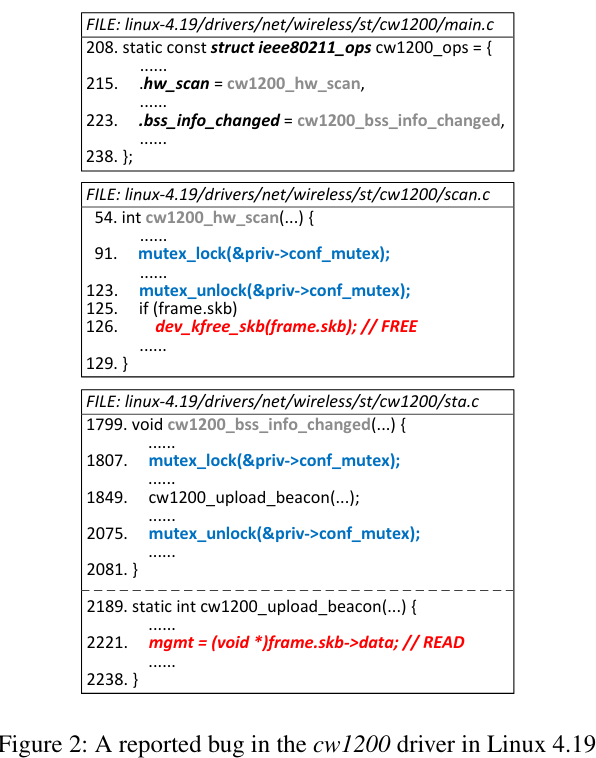
\includegraphics[height=0.9\textheight]{../betterpl/linux-conc-uaf-fig}
};
\node[anchor=north west,font=\small,align=left] at (fig.north east) {
Figure from Bai, Lawall, Chen and Mu \\ (Usenix ATC'19) \\
{\scriptsize ``Effective Static Analysis of Concurrency} \\ {\scriptsize Use-After-Free Bugs in Linux drivers''} \\
~ \\
bug in a wireless networking driver
};
\end{tikzpicture}
\end{frame}


\subsection{other Rust smart pointers}

\begin{frame}{other policies Rust supports}
    \begin{itemize}
        \item \myemph<2>{RefCell} --- borrowing, but check at runtime, not compile-time
            \begin{itemize}
            \item detect at runtime if used while already used
            \item internally: destructor call when returned object goes out of scope
            \end{itemize}
        \item Weak --- reference-counting, but don't contribute to count
            \begin{itemize}
            \item detect at runtime if used with count = 0
            \end{itemize}
        \item Mutex --- with multicore, enforce one user at a time by waiting
        \item \ldots
    \end{itemize}
\end{frame}




\subsection{exercise: smart pointer use case}
\begin{frame}{exercise: which smart pointer?}
    \begin{itemize}
    \item Rc, Arc (reference counting, w/ or w/o threading support
    \item RefCell (borrowing, check at runtime)
    \item Weak (reference counting, but don't contribute to count --- works with Rc)
    \item Mutex (with multicore, one-at-a-time by waiting)
    \vspace{.5cm}
    \item say I have flight reservation system with Flight objects that have
        references to Ticket objects and vice-versa, \\
        and Customer objects that have references to Ticket objects and vice-versa?
    \end{itemize}
\end{frame}


\section{zero-overhead}

\begin{frame}{zero-overhead}
    \begin{itemize}
    \item normal case --- lifetimes --- have no overhead
    \item compiler proves safety, generates code with no bookkeeping
        \vspace{.5cm}
    \item other policies (e.g. reference counting) do
    \item \ldots but can implement new ones if not good enough
    \end{itemize}
\end{frame}



\section{aside: other language enforcement?}
\begin{frame}{other things languages can enforce?}
    \begin{itemize}
    \item saw: enforcing no use-after-free
    \item lots of coding conventions we might try to enforce:
    \vspace{.5cm}
    \item code's runtime does not depend on secret data
        \begin{itemize}
        \item secret data has different type
        \item variable time operations prohibited with secret data
        \end{itemize}
    \item sensitive data not passed to wrong place
        \begin{itemize}
        \item sensitive data has different type
        \item assignment to wrong places is a type error
        \end{itemize}
    \item code has bounded runtime
        \begin{itemize}
        \item langauge prohibits not unbounded loops, recursion, etc.
        \end{itemize}
    \end{itemize}
\end{frame}


\subsection{example: constant time languages}
\begin{frame}{some constant time ideas}
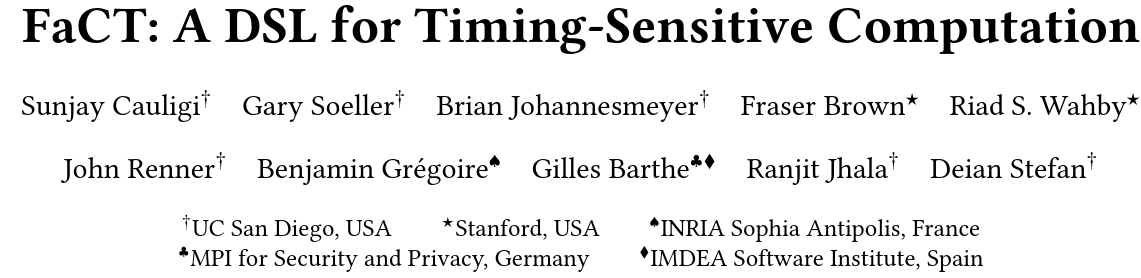
\includegraphics[width=0.8\textwidth]{../betterpl/fact-title}
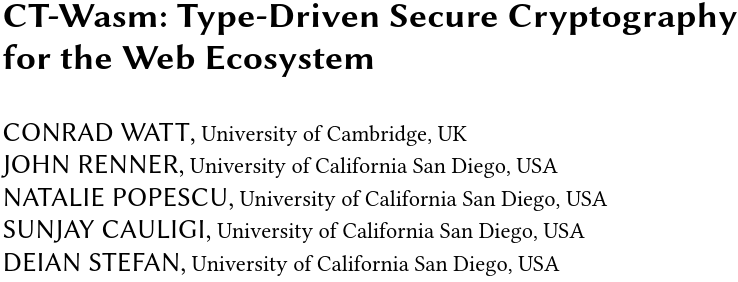
\includegraphics[width=0.8\textwidth]{../betterpl/ct-wasm-title}
\begin{itemize}
\item FaCT, PLDI 2019; CT-Wasm: POPL 2019
\end{itemize}
\end{frame}

\begin{frame}{constant-time programming languages}
    \begin{itemize}
    \item active research area, no consensus on what works best
    \vspace{.5cm}
    \item common approach: separate type for \textbf{secret} data
    \item compiler or language virtual machine disallows variable-time operations using secret data
    \item no secret-based array lookup (cache timing varies)
        \begin{itemize}
        \item e.g. array[secret\_value] $\rightarrow$ compile error (type mismatch)
        \end{itemize}
    \item no secret-based integer division (usually variable speed instruction)
    \item \ldots
    \vspace{.5cm}
    \item explicit operations for any secret-to-non-secret conversions
    \end{itemize}
\end{frame}


\section{principle: least privilege}

\begin{frame}{least privilege}
    \begin{itemize}
    \item a typical program I run on my desktop is allowed to\ldots
    \item make network connections to anywhere
    \item upload all my files to the Internet
    \item delete all my files
    \item record all my keystrokes
    \item \ldots
    \vspace{.5cm}
    \item but it probably doesn't need to\ldots
    \item ideally: if typical program was compromised/malicious, \\
          it still wouldn't be able to do most of these things
    \end{itemize}
\end{frame}



\subsection{what do browsers need?}

\begin{frame}{things applications need?}
    \begin{itemize}
    \item what things should browser be able to do?
    \item what things should word processor be able to do?
    \end{itemize}
\end{frame}

\begin{frame}{things broswers need}
    
\includegraphics[width=.5\textwidth]{../sandbox/savelinkas}
    \begin{itemize}
        \item save files
        \item have your webmail password
        \item \ldots
    \end{itemize}
\end{frame}


\subsection{OS users}

\begin{frame}<1>[fragile,label=multiOS]{multi-user OSs}
\lstset{
    language={},style=small,
    moredelim={**[is][\color{red!70!black}]{~in~}{~end~}},
}
\begin{lstlisting}
cr4bd@labunix01:~$ ~in~cp myprogram.exe /bin/ls~end~
cp: cannot create regular file ‘/bin/ls’: Permission denied
\end{lstlisting}
    \begin{itemize}
        \item programs have \myemph{limited privileges}
        \item<2-> OS tracks ``user'' of running every program
        \item<2-> result: malware I installed shouldn't be able to effect other users
        \item<2-> idea 1: reuse this support for web browsers
            \begin{itemize}
            \item webpage should run as ``different user''
            \item malware should only affect web browser?
            \end{itemize}
    \end{itemize}
\end{frame}

\begin{frame}[fragile,label=permEnforce]{permission enforcement}
    \begin{minted}[fontsize=\small]{C}
struct Process {
    int user_id;
    ...
};
int handle_open_system_call(char *filename, ...) {
    Process* currentProcess = GetCurrentProcess();
    File* file = GetFileByFilename(filename);
    if (!file->UserCanAccess(currentProcess->user_id)) {
        return ERROR_PERMISSION_DENIED;
    }
    ...
}
\end{minted}
\end{frame}

\againframe<2>{multiOS}



\subsection{promise: privilege separation}

\begin{frame}{the privilege separation idea}
    \begin{itemize}
    \item can't make whole browser run as ``different user''
        \begin{itemize}
        \item still need to save files, read password, etc.
        \end{itemize}
    \item how about just the parts that are ``dangerous''?
        \begin{itemize}
        \item part that runs scripts, parses HTML
        \end{itemize}
    \end{itemize}
\end{frame}




\section{privilege separation: video decode}

\begin{frame}{simple privilege separation}
    \begin{itemize}
    \item simple example: want to show videos
    \item video decoding library is tens of thousands of lines of code
        \begin{itemize}
        \item often buggy, includes hard-to-check hand-written assembly
        \end{itemize}
    \item what does video decoding library do?
        \begin{itemize}
        \item read video file as input
        \item output images as output
        \end{itemize}
    \end{itemize}
\end{frame}

\begin{frame}{simple privilege seperation}
    \begin{itemize}
    \item setup: create new user
    \item start video decoder as new user
    \item communicate via ``pipes''
        \begin{itemize}
        \item like terminal to be used by program
        \end{itemize}
    \end{itemize}
\end{frame}

\begin{frame}[fragile,label=privSepOutline]{simple privilege seperation}
\begin{minted}[fontsize=\fontsize{10}{10}]{C}
/* dangerous video decoder to isolate */
int main() {
    /* switch to right user */
    SetUserTo("user-without-privileges"));
    while (fread(videoData, sizeof(videoData), 1, stdin) > 0) {
        doDangerousVideoDecoding(videoData, imageData);
        fwrite(imageData, sizeof(imageData), 1, stdout);
    }
}

/* code that uses it */
    FILE *fh = RunProgramAndGetFileHandle("./video-decoder");
    for (;;) {
        fwrite(getNextVideoData(), SIZE, 1, fh);
        fread(image, sizeof(image), 1, fh);
        displayImage(image);
    }
\end{minted}
\end{frame}




\subsection{another user is not enough}

\begin{frame}{issues with privilege separation (1)}
    \begin{itemize}
    \item ``other user'' can still do too much
    \vspace{.5cm}
    \item read unprotected files
        \begin{itemize}
        \item most of them?
        \end{itemize}
    \item write temporary files?
    \item open network connections
    \item use all your memory
    \item \ldots
    \end{itemize}
\end{frame}




\subsection{awkwardness of creating a new user}

\begin{frame}{issues with privilege separation (2)}
    \begin{itemize}
    \item awkward to do
    \item switching users requires special permissions
    \item seperate user for \myemph{each} video decoder, audio decoder, web page renderer?
        \begin{itemize}
        \item users can debug processes from same user
        \end{itemize}
    \item slowdown --- extra copying
    \end{itemize}
\end{frame}



\section{system calls as OS interface}
\begin{frame}{program to OS interface}
    \begin{itemize}
    \item primary way application talks to OS: system calls
    \vspace{.5cm}
    \item function calls that request OS do something
    \item typically: how program can interact with rest of system
        \begin{itemize}
        \item files
        \item other programs
        \item the network
        \item devices
        \item\ldots
        \end{itemize}
    \vspace{.5cm}
    \item controlling program behavior: control what system calls
    \end{itemize}
\end{frame}


\section{simple Linux system call filtering}
\newmintinline{C}{}
\begin{frame}{Linux system call filtering API}
    \begin{itemize}
    \item privilege seperation support: system call filtering
    \item simple API: \Cinline|seccomp(SECCOMP_SET_MODE_STRICT, 0, 0)|
        \vspace{.5cm}
            \item ``The only system calls the calling thread is permitted to make are \texttt{read},
                \texttt{write}, \texttt{\_exit}, and \texttt{sigreturn}. Other system calls [kill
                the program].''
            \item read/write only work on \myemph{already open files}
    \vspace{.5cm}
    \item later: what if we want to be finer-grained?
    \end{itemize}
\end{frame}


\section{definition: sandbox}
\begin{frame}{``sandboxing''}
    \begin{itemize}
    \item result of filtering operations called a ``sandbox''
    \item idea: attacker can play in sandbox as much as they want
    \item can't do anything ``harmful''
    \vspace{.5cm}
    \item other possible implementations:
        \begin{itemize}
        \item e.g. virtual machine
        \end{itemize}
    \end{itemize}
\end{frame}




\section{Chrome architecture}
\usetikzlibrary{positioning,shapes.callouts}

\begin{frame}{Chrome architecture}
    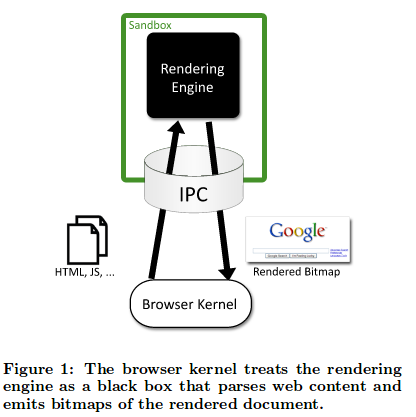
\includegraphics[height=0.8\textheight]{../sandbox/chrome-arch}
\end{frame}

\begin{frame}{talking to the sandbox}
    \begin{itemize}
    \item browser kernel sends commands to sandbox
    \item sandbox sends commands to browser kernel
    \item idea: commands only allow necessary things
    \end{itemize}
\end{frame}

\begin{frame}{original Chrome sandbox interface}
    \begin{itemize}
        \item sandbox to browser ``kernel''
            \begin{itemize}
                \item show this image on screen
                \begin{itemize}
                    \item (using shared memory for speed)
                \end{itemize}
            \item \myemph<2-3>{make request\tikzmark{request} for this URL}
            \item \myemph<4>{download\tikzmark{download} files to local FS}
            \item \myemph<5>{upload\tikzmark{upload} user requested files}
            \end{itemize}
        \item browser ``kernel'' to sandbox
            \begin{itemize}
                \item send user input
            \end{itemize}
    \end{itemize}
    \begin{tikzpicture}[overlay,remember picture]
        \coordinate (middle) at ([yshift=-1cm]current page.center);
        \begin{visibleenv}<2>
            \node[my callout=request,anchor=center,align=center]  at (middle) {
                needs filtering --- at least no \texttt{file:} (local file) URLs
            };
        \end{visibleenv}
        \begin{visibleenv}<3>
            \node[my callout=request,anchor=center,align=center] at (middle) {
                can still read any website! \\
                still sends normal cookies!
            };
        \end{visibleenv}
        \begin{visibleenv}<4>
            \node[my callout=download,anchor=center,align=center] at (middle) {
                files go to download directory only \\
                can't choose arbitrary filenames
            };
        \end{visibleenv}
        \begin{visibleenv}<5>
            \node[my callout=upload,anchor=center,align=center] at ([yshift=-1cm]middle) {
                browser kernel displays file choser \\
                only permits files selected by user
            };
        \end{visibleenv}
    \end{tikzpicture}
\end{frame}



% FIXME: Chrome Site Isolation
\subsection{Site Isolation}
% https://www.usenix.org/conference/usenixsecurity19/presentation/reis

\begin{frame}{Site Isolation}
\begin{itemize}
\item Chrome since version 67 (desktop)/77 (Mobile) has process per site
\item site $\approx$ registered domain name (example.com, example.co.uk, etc.)
    \begin{itemize}
    \item slightly different than same origin policy
    \end{itemize}
\vspace{.5cm}
\item complicated to implement:
    \begin{itemize}
    \item single web page can embed content from multiple other sites
        \begin{itemize}
        \item and those other sites can embed content from yet more sites
        \end{itemize}
    \item web page can call services on other websites with ``permission'' of other website
    \item clicking link may or may not requiring switching to new process
    \end{itemize}
\vspace{.5cm}
\item same separation being prototyped in recent Firefox builds
\end{itemize}
\end{frame}


\section{OpenSSH architecture}
\begin{frame}{OpenSSH privilege seperation}
    \begin{itemize}
    \item OpenSSH uses privilege seperation for its SSH server
    \item what runs on the lab machines when you log into them
    \vspace{.5cm}
    \item separate network processing code from authentication code
    \item seperate process per connection --- users don't share
    \vspace{.5cm}
    \item developed before system call filtering was widely available
        \begin{itemize}
        \item uses separate user + chroot (we'll talk later) to isolate
        \end{itemize}
    \end{itemize}
\end{frame}

\begin{frame}{OpenSSH privsep protocol}
    \begin{itemize}
    \item sandboxed process tells ``monitor'' to:
        \vspace{.25cm}
    \item perform \myemph{cryptographic operations}
        \begin{itemize}
        \item long-term keys never in sandboxed process
        \item commands to ask for cryptographic messages they need
        \end{itemize}
    \item ask to switch to user --- if given user password, etc.
        \begin{itemize}
            \item \myemph{monitor process verifies} login information
        \end{itemize}
    \item after authentication: new process running as logged-in user 
        \begin{itemize}
            \item (normally) no issues with special privileges
        \end{itemize}
    \end{itemize}
\end{frame}


\begin{frame}{privilege seperation overall}
    \begin{itemize}
    \item large application changes
        \begin{itemize}
        \item OpenSSH: 3k lines of code for communication/etc. added
        \item OpenSSH: 2\% of existing code (950 of 44k lines) changed
        \item (but most changes simple)
        \end{itemize}
    \item lots of application knowledge
        \begin{itemize}
        \item what is a meaningful separation of `privileged' and `unprivileged'?
        \end{itemize}
    \item better application design anyways?
    \end{itemize}
\end{frame}



\subsection{exercise: priv sep for}
\begin{frame}{privilege separation for}
    \begin{itemize}
    \item let's say we wanted to add sandboxing/privilege separation to an (standalone) mail program
    \vspace{.5cm}
    \item exercise 1: where would be concerned about security problems?
    \item exercise 2: propose a way of dividing up the program
    \end{itemize}
\end{frame}


\section{normal application confinement?}
\begin{frame}{application confinement}
    \begin{itemize}
    \item confining whole browsers was hard
        \begin{itemize}
            \item we trust them to do a lot of things --- e.g. write arbitrary files
        \end{itemize}
    \item but maybe we can do this for simpler applications?
    \item idea 1: applications send system calls to OS 
        \begin{itemize}
        \item \myemph{limit syscalls} like we limited browser kernel commands
        \item constructing command language ``in reverse''
        \end{itemize}
    \end{itemize}
\end{frame}



\subsection{more fine-grained filtering?}
\begin{frame}{Linux system call filtering: detailed}
    \begin{itemize}
    \item Linux supports more fine-grained system call filtering
    \item using BPF (Berkeley Packet Filter) programming language
        \begin{itemize}
        \item compiled in the kernel to assembly to check system calls
        \end{itemize}
    \vspace{.5cm}
    \item can check system call argument values, but\ldots
        \begin{itemize}
        \item problems with pointer arguments
        \item too many system calls
        \end{itemize}
    \end{itemize}
\end{frame}

\begin{frame}[fragile,label=open]{Linux system call: open}
\begin{lstlisting}[language=C,style=small]
open("foo.txt", O_RDONLY);
\end{lstlisting}
\begin{itemize}
\item parameters:
    \begin{itemize}
    \item system call number: 2 (``open'')
    \item argument 1: 0x7fffe983 (address of string ``foo.txt'')
    \item argument 2: 0 (value of ``\texttt{O\_RDONLY}'')
    \end{itemize}
\item very problematic to filter using BPF interface
\vspace{.5cm}
\item can deal with using `ptrace' --- Linux debugging interface
    \begin{itemize}
    \item BPF can trigger something like a debugger breakpoint
    \item breakpoint wakes up monitor program (attached like debugger)
    \item `monitor' program can perform system call on program's behalf
    \end{itemize}
\end{itemize}
\end{frame}

\begin{comment}
\begin{frame}[fragile,label=openRuleP1]{lots of ways to open (1)}
\begin{itemize}
\item let's say we want to disallow:
\end{itemize}
\begin{lstlisting}[language=C,style=smaller]
open("/dev/keyboard", O_RDONLY);
\end{lstlisting}
\begin{itemize}
\item problem 1: some other ways of doing that?
\begin{lstlisting}[language=C,style=smaller]
chdir("/dev");
open("keyboard, O_RDONLY);

open("../../../../../../dev/keyboard", O_RDONLY);

symlink("/dev", "/tmp/foo");
open("/tmp/foo/keyboard", O_RDONLY);
\end{lstlisting}
\end{frame}

\begin{frame}[fragile,label=openRuleP2]{lots of ways to open (2)}
\begin{itemize}
\item let's say we want to disallow:
\end{itemize}
\begin{lstlisting}[language=C,style=smaller]
open("/dev/keyboard", O_RDONLY);
\end{lstlisting}
\begin{itemize}
\item problem 2: filter language doesn't allow reading pointers
    \begin{itemize}
    \item string is passed via pointer
    \end{itemize}
\item problem 3: string can be changed from another core
    \begin{itemize}
    \item between when filter runs and when syscall runs
    \end{itemize}
\end{itemize}
\end{frame}

\begin{frame}[fragile,label=openRuleP3]{lots of ways to open (3)}
\begin{itemize}
\item let's say we want to disallow:
\end{itemize}
\begin{lstlisting}[language=C,style=smaller]
open("/dev/keyboard", O_RDONLY);
\end{lstlisting}
\begin{itemize}
\item problem 4: several other syscalls (that might be used innocently)
    \begin{itemize}
    \item openat, open\_by\_handle\_at
    \item would need to write additional filter rules
    \item \ldots or break programs that aren't trying to violate rule
    \end{itemize}
\end{itemize}
\end{frame}

\begin{frame}[fragile,label=howManySystemCalls]{Linux system calls}
\begin{itemize}
\item x86-64 linux: \myemph{313 system calls}
\item opening a file:
    \begin{itemize}
    \item open (number 2)
    \item openat (number 257)
    \item open\_by\_handle\_at (number 304)
    \end{itemize}
\item coordinating between threads (for using multiple cores):
    \begin{itemize}
    \item rt\_sigaction (number 13)
    \item rt\_sigprocmask (number 14)
    \item rt\_sigreturn (number 15)
    \item tkill (number 200)
    \item futex (number 202)
    \item set\_robust\_list (number 273)
    \item get\_robust\_list (number 274)
    \item more?
    \end{itemize}
\end{itemize}
\end{frame}
\end{comment}


\end{document}
